\section{Fundamental Scheduling Patterns}

%% In this paper, we require that the push, pop, and peek rates of each
%% filter are known at compile time.  This enables the compiler to
%% calculate a steady-state for the stream graph: a repetition of each
%% filter that does not change the number of items buffered on any data
%% channel~\cite{lee87,karczmarek:lctes:2003}. In combination with a
%% simple program analysis that estimates the number of operations
%% performed on each invocation of a given work function, the
%% steady-state repetitions offer an estimate of the work performed by a
%% given filter as a fraction of the overall program execution.  This
%% estimate is important for our software pipelining technique.

There is a complex space of trade-offs to explore when devising a
schedule. What we show in this section is that scheduling decisions
can be broken down to reasoning about simple stream graph
patterns. The simple decomposition of stream graphs into these
patterns facilities more scheduling freedom and better efficiency for
a static scheduler. We will show later that a static scheduler that
makes use of these patterns yields results that are comparable to
a dynamic scheduler.

We present several primitive scheduling patterns. Each of the patterns
represents a small stream graph consisting of one or two actors. The
patterns distinguish between stateless and stateful actors. A
stateless actor does not maintain any internal state that is modified
from one firing to the next. A stateless actor is essentially a data
parallel actor, whereas a stateful actor requires a serialization of
its firings so that its internal state is always consistent.  For each
pattern, we illustrate how to construct a {\it maximum efficiency
static schedule} (MESS) for {\it two} parallel processors.

A static schedule for our purposes simply makes decisions on the
assignment of actors to processors and the ordering of actor firings
within a processor. The dynamic actor firings are guarded by the
dataflow dependencies, and such dependences are the only
synchronization mechanisms required for proper execution.
%%Without loss
%%of generality, we assume that all actors consume and produce an equal
%%number of data items per firing...
This is different from a full dynamic scheduler which also must decide
on the assignment and ordering of actors, or full static schedulers
that require synchronization barriers or explicit binding of actor
firings to time slots. The combination of static
assignment and ordering with dynamic issue offers a scalable solution
for multicore architectures.

The patterns themselves were initially inspired by observations
derived from studying the characteristics of streaming application. We
believe that in their current formulation, they present a foundation
to further explore the complex space of scheduling tradeoffs for
static and dynamic paradigms alike.  We believe that its is possible
to further extend the pattern-based scheduling methodology using a
recursive composition of the patterns to schedule larger stream graphs
on a larger number of processors.

\begin{table*}[t]
\center
\caption{\small Maximum efficiency static schedules for the stream graph patterns.}
{\small
\begin{tabular}{|c|c|c|c|} \hline
                 & {\bf bottleneck} & ${\bf P_1}$  & ${\bf P_2}$ \\ \hline
{\bf Pattern 1}  & ---              & $A$     & $A$ \\ \hline
{\bf Pattern 2}  & ---              & $A$     & --- \\ \hline
{\bf Pattern 3}  & ---              & $A, B$  & $A, B$ \\ \hline
{\bf Pattern 4}  & ---              & $A$     & $B$ \\ \hline
{\bf Pattern 5}  & $W_A \le W_B$    & $A$     & $B$ \\ \cline{2-4}
                 & $W_A > W_B$      & $(W_A - W_B) A, (2W_A) B$ & $(W_A + W_B) B$ \\ \hline
{\bf Pattern 6}  & $W_A \ge W_B$    & $A$     & $B$ \\ \cline{2-4}
                 & $W_A < W_B$      & $(2W_B) A, (W_B - W_A) B$ & $(W_A + W_B) B$ \\ \hline
{\bf Pattern 7}  & $W_A \le W_B$    & $A$     & $B$ \\ \cline{2-4}
                 & $W_A > W_B$      & $(W_A - W_B) A, (2W_A) B$ & $(W_A + W_B) B$ \\ \hline
{\bf Pattern 8}  & ---              & $A$     & $B$ \\ \hline
\end{tabular}}
\label{tab:pattern-sched}
\end{table*}


\begin{figure}[t!]
\begin{center}
\psfig{figure=patterns.eps,height=4.5in}
\caption{{\small The 8 patterns.
\protect\label{fig:patterns}}}
\end{center}
\end{figure}

\subsection{Pattern 1: Singular Data-Parallel Actor}

The simplest pattern is shown in Figure~\ref{fig:patterns}a. It
represents a singular {\it stateless} actor $A$ that consumes no
input, and produces no output.
%%and requires $W_A$ units of work to execute
This patterns is trivial to schedule statically for two
processors. Since the actor is stateless, and has no dependences, each
of the two processors executes an instance of $A$ as shown Table~\ref{tab:pattern-sched}.

\subsection{Pattern 2: Singular Stateful Actor}

A related pattern is shown in Figure~\ref{fig:patterns}b. It
represents a singular {\it stateful} actor $A$ that consumes no input
and produces no output.
%%, and requires $W_A$ units of work to execute.
This patterns is also trivial to schedule statically. Since there is a
dependence between each of the actor firings, the only feasible
schedule is to sequentially execute the actor on a single
processor. The binding of the actor to a specific and unique
processor avoids inter-processor synchronization and
potentially costly communication to mutate the state of the actor
appropriately between processors.

\subsection{Pattern 3: Data-Parallel Pipeline}

The third pattern is shown in Figure~\ref{fig:patterns}c. It consists
of two actors $A\rightarrow B$ connected through a FIFO to form a two
stage {\it pipeline}. Both of the actors are stateless, and hence data
parallel. In this pattern, the maximum efficiency schedule runs one
instance of the pipeline on processor $P_1$ and another independent
instance of the pipeline on the second processor $P_2$.  This schedule
requires no synchronization between processors.

\subsection{Pattern 4: Stateful Pipeline}

The fourth pattern is shown in Figure~\ref{fig:patterns}d. It is
similar to the previous pattern with the distinction that the actors
in the pipeline $A\rightarrow B$ are stateful. The maximum efficiency
schedule for this pattern is to place one actor on one processor and
the other on the second processor. This requires synchronization
between the two processors in terms of data exchange along the FIFO
channel. In other words, an instance $i$ of actor $B$ can not execute
until instance $i$ of actor $A$ has completed its execution.  

\subsection{Pattern 5: Mixed Mode Pipeline with Stateless Source}

The fifth pattern is shown in Figure~\ref{fig:patterns}e. It is a
pipeline $A\rightarrow B$ where actor $A$ is stateless and actor $B$
is stateful. In this pattern, the characteristics of the work required
to execute $A$ and $B$ can lead to different maximal efficiency
schedules.  There are two cases. First, if $W_A \le W_B$ then the
schedule is bottlenecked by the stateful actor and the best schedule
is the same as the one derived for Pattern~4. However, if the
bottleneck is the stateless actor, then there is an opportunity to
exploit the data parallelism in the stateless actor to balance the
work between the two actors.

This fifth pattern (and as will be apparent shortly in the following
pattern) leads to a unique and elegant MESS that has a closed form
solution. Consider the simple case where $A$ produces a single item
per firing, and $B$ consumes a single item per firing, and let $W_A =
2$ units of work and $W_B = 1$ unit of work. Intuitively, to maximize
utilization of the two processors, first we require that the total
work done in a steady state by $P_1$ is equal the work done by
$P_2$. In other words, it is necessary for the two processors to be
properly load balanced. Furthermore, to minimize synchronization
overhead, the stateful actors should be collocated on the same
processor. Lastly, the schedule should maximize the decoupling between
the two processors by assigning the greatest possible number of
stateless actors to the processor where the stateful actor is not
assigned.

In the domain of instruction scheduling, if $A$ and $B$ are
instructions in a loop, then unrolling the loop exposes more
instruction level parallelism that allows a compiler to hide the
latency of either instruction. Coarse grained software
pipelining~\cite{mgordon-aplos06} has a similar effect. Thus
conceptually unrolling the simple pipeline in this example by a factor
of 4 leads to a schedule that is perfectly load balanced as show in
Figure~\ref{fig:pattern5-sched}. 

A generalization of this example that satisfies the MESS desiderata
for this schedule thus maximizes the firings of $A$ on $P_2$ such that
the two processors are load balanced and the total number of $A$ and
$B$ actor firings is the same. It turns out that it is possible to
construct such a schedule readily for any value of $W_A < W_B$ using
the closed form solution we report in
Table~\ref{tab:pattern-sched}. It is trivial to show that both
processors are load balanced for any $W_A > W_B$. The total work done
on $P_1$ is equal to
\[
(W_A - W_B) \cdot W_A + (2 \cdot W_A) \cdot W_B
\]
and similarly the work done on $P_2$ equals
\[
(W_A + W_B) \cdot W_A
\]
and both equations reduce to 
\[
(W_A)^2 + (W_A \cdot W_B)
\]
in terms of total work per steady.

The closed form scheduling solution for this pattern (and similarly
the pattern described next) suggests that with adequate work
estimation for the actor firings, it is feasible to statically
construct a schedule that achieves a utilization that is comparable to
a dynamic scheduler.

\subsection{Pattern 6: Mixed Mode Pipeline with Stateful Source}

The sixth pattern is also a pipeline $A\rightarrow B$ but in this case
actor $A$ is stateful and actor $B$ is stateless. This pattern is
illustrated in Figure~\ref{fig:patterns}f. There are many similarities
between this pattern and the previous pattern, and there is a closed
form scheduling solution for this pattern as well. 

When the pipeline is bottlenecked by the stateful actor ($W_A \ge
W_B$), there is not any scheduling freedom and the best possible
schedule is to assign each actor to its own processor. However when
the stateless actor is the bottleneck ($W_A < W_B$), it is possible to
hide its latency by adequately buffering the data between the two
actors. A MESS for this pattern that satisfies the same desiderata as
those in Pattern 5 leads to the schedule illustrated in
Figure~\ref{fig:pattern6-sched} when $W_A = 1$ and $W_B = 2$.  A
generalization of this example leads to the closed form scheduling
solutions shown in Table~\ref{tab:patterns-sched} for any $W_A < W_B$.


\subsection{Pattern 7: Mixed Mode Explicitly Parallel Actors}

Unlike the previous patterns which addressed pipeline composition of
actors, this patterns shown in Figure~\ref{fig:patterns}g addresses
explicit concurrency between actors that are not in a direct
producer-consumer relationship, and one of the actors ($A$) is
stateless and the other ($B$) stateful. As it turns out, the
scheduling pattern in this case follows that of a previous pattern
(Pattern 5), with the exception that no buffers are shared between the
two actors. Hence the only consideration that a static scheduler  is
cognizant of is the load balancing of work across the two
processors. When $W_A \le W_B$ the schedule is trivial: each actor is
assigned to a unique processor. When $W_A > W_B$, the scheduling
pattern is the same as that for Pattern 5.

\subsection{Pattern 8: Stateful Explicitly Parallel Actors}

The final pattern that we consider is shown in
Figure~\ref{fig:patterns}h. It is similar to the previous patterns but
in this case both actors are stateful. The schedule in this case is
trivial to construct and simple assigns each actor to a unique
processor.

\subsection{Complex Patterns}

%% \begin{figure}[t]
%% \begin{center}
%%  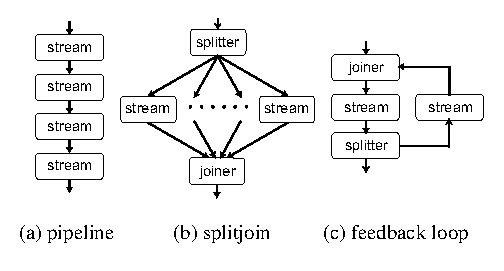
\includegraphics[scale=1, angle=0]{./constructs-eg.eps}
%%  \caption{Examples of hierarchical streams.}
%%  \label{fig:containers}
%% \end{center}
%% \end{figure}

%% We assume there are three fundamental primitives for hierarchically
%% composing actors into larger stream graphs. They are shown in
%% Figure~\ref{fig:containers}. A {\it pipeline} connects streams
%% sequentially, as we have already described. A {\it splitjoin}
%% specifies independent and parallel streams that diverge from a common
%% {\it splitter} and merge into a common {\it joiner}. The final
%% hierarchical primitive is a {\it feedbackloop} that provides a way to
%% create cycles in the graph. The structured composition of actors into
%% stream graphs using these primitives simplifies the scheduling space
%% for a static scheduler. 
There are other more complex patterns that arise in streaming
applications. However we have found that it is practical to refine
large and complex stream graphs to simple and more natural scheduling
patterns. Our experience with the set of streaming benchmarks we
evaluate is that this is a practical approach that yields good overall
performance. More intelligent ways to handle the composition of the
patterns present an interesting and challenging topic, and are beyond
the scope of this paper.


